\documentclass[a4paper,12pt]{report}
\usepackage[spanish]{babel}             % Para escribir en español
\usepackage{mathptmx}                   % Usa Times (parecida a Times New Roman)
\usepackage{setspace}                   % Para interlineado
\onehalfspacing                         % Establece interlineado 1.5
\usepackage{xcolor}                     % Para colores personalizados
\usepackage[table]{xcolor}              % Para los colores en las tablas
% \usepackage[table,xcdraw]{xcolor}     % Para incluir opciones de color en la tabla
\usepackage{graphicx}                   % Para incluir imágenes
\usepackage{pdfpages}                   % Para incluir pdf
\usepackage{geometry}                   % Para ajustar márgenes
\usepackage{titlesec}                   % Para personalizar títulos
\usepackage{fancyhdr}                   % Para encabezados y pies de página
\usepackage{hyperref}                   % Para incluir URLs
\usepackage{csquotes}                   % Para las citas inline 
\usepackage[backend=bibtex]{biblatex}   % Para añadir bibliografía con BibLaTeX
\usepackage{float}                      % Para las tablas

% Configuración de márgenes
\geometry{left=3cm, right=3cm, top=2.5cm, bottom=2.5cm}
\graphicspath{{resources/}{../pdf/}}

% Personalización de títulos
\titleformat{\chapter}[display]
  {\Huge\bfseries}{}{0pt}{\Huge}

% Encabezados y pies de página
\pagestyle{fancy}
\fancyhead{}
\fancyfoot{}
\fancyfoot[C]{\thepage}

% Partición de palabras en textos justificados
\hyphenation{je-fa-tu-ra}
\hyphenation{LABORA}
\hyphenation{ma-nu-fac-tu-ra}
\hyphenation{pro-fe-sio-nal}
\hyphenation{pro-fe-sio-na-les}
\hyphenation{co-rres-pon-dien-tes}
\hyphenation{pro-xi-mi-da-des}

% Indicar ficheros con la bibliografía
\addbibresource{biblio.bib}

% Configuración de hipervínculos
\hypersetup{
    colorlinks=true,
    linkcolor=black,    % Enlaces internos (a secciones, figuras, etc.)
    urlcolor=gray,      % Enlaces externos (URLs)
    citecolor=black,    % Referencias/citas
    pdftitle={Memoria Prácticum II},
    pdfauthor={Nombre Apellido},
    pdfsubject={Prácticas en centro educativo}
}

\begin{document}
    \begin{titlepage}
    \begin{center}
        \vspace*{2cm}
        
        
\includegraphics[width=0.5\textwidth]{resources/logo_ua.png}\\[1cm]
        
        \textcolor{gray}{\Huge \textbf{Memoria del Prácticum II}}\\[1cm]
        \rule{10cm}{0.4mm} \\[1cm]
        
        {\Large Máster en Profesorado de Educación Secundaria Obligatoria y Bachillerato, Formación Profesional y Enseñanza de Idiomas}\\[1cm]
        
        \textbf{Especialidad:} Especialidad 3. Formación Profesional Cuerpo Técnico\\[0.5cm]
        \textbf{Alumno/a:} Lorena González Núñez de Arenas\\[0.5cm]
        \textbf{Curso académico:} 2024-2025\\[0.5cm]
        \textbf{Centro de Prácticas:} CIPFP Canastell\\[0.5cm]
        \textbf{Tutor/a del centro:} Antonio Verdejo Borja\\[0.5cm]
        \textbf{Tutor/a de la Facultad:} Raúl Gutierrez Fresneda\\[0.5cm]
        
        \vfill
        \textcolor{gray}{\Large \textbf{Universidad de Alicante}}\\
        \textcolor{gray}{Facultad de Educación}\\
        \textcolor{gray}{San Vicente del Raspeig, Alicante}\\
        \textcolor{gray}{Fecha: \today}
    \end{center}
\end{titlepage}
    % Declaración de Responsabilidad
\newpage
\section*{DECLARACIÓN DE RESPONSABILIDAD Y AUTORÍA}
D/Dª.: Lorena González Núñez de Arenas, con DNI 48620705Q, 
estudiante del Máster universitario en profesorado de educación secundaria obligatoria y bachillerato, formación profesional y enseñanza de idiomas, 
de la Universidad de Alicante, realizado en el período del 20 de enero de 2025 al 20 de febrero de 2025. \\


DECLARA QUE:\\
La Memoria del Prácticum denominado\\
Memoria del Prácticum I\\
ha sido desarrollado respetando los derechos intelectuales de terceros, conforme las citas que 
constan en las páginas correspondientes y cuyas fuentes se incorporan en la bibliografía, así 
como cualquier otro derecho, por ejemplo de imagen que pudiese estar sujeto a protección 
del copyright.\\

En virtud de esta declaración, afirmo que este trabajo es inédito y de mi autoría, por lo que me 
responsabilizo del contenido, veracidad y alcance de la Memoria del Prácticum, y asumo las consecuencias administrativas y jurídicas 
que se deriven en caso de incumplimiento de esta declaración.\\

Para que así conste, firmo la presente declaración en \\
Alicante, a \today. \\

Fdo.:  \
\vspace{10\baselineskip}\

Este documento formará parte de la memoria de los Practicum o TFG o TFM correspondiente y 
será la primera página de los mismos.\\

\textsuperscript{*}	\textit{Documento aprobado en Junta de Facultad el 19 de octubre de 2017.}\\


    \renewcommand{\contentsname}{Índice}
    \tableofcontents
    \newpage

    % RESUMEN
\chapter{Resumen}

Esta memoria recoge la experiencia y las intervenciones realizadas durante el Prácticum II en el CIPFP Canastell, dentro del módulo de \textit{Instalaciones Domóticas} del segundo curso del Grado Medio en Instalaciones Eléctricas y Automáticas. La intervención se centró en una situación de aprendizaje que abordó los riesgos de seguridad en la domótica de bajo coste, permitiendo al alumnado analizar vulnerabilidades en dispositivos IoT y aplicar buenas prácticas de ciberseguridad.

A lo largo del período de prácticas, mi rol principal fue de observadora, ya que mi formación en Ingeniería Informática no estaba alineada con el contenido eléctrico del ciclo. Sin embargo, esto no impidió que pudiera desarrollar una intervención concreta en un área más afín a mi perfil: la seguridad en domótica de bajo coste. 

La situación de sprendizaje titulada "Domótica de Bajo Coste: ¿Comodidad Inteligente o Riesgo Silencioso?", se llevó a cabo el 6 de febrero de 2025. En esta sesión, el alumnado analizó vulnerabilidades de dispositivos IoT de bajo coste y aplicó buenas prácticas en ciberseguridad. La actividad combinó una parte teórica donde se explicaron los riesgos y ataques más comunes en redes domóticas, y una parte práctica en aula-taller, en la que los estudiantes experimentaron con la configuración y seguridad de un \textit{enchufe inteligente Shelly Plug} y un \textit{router WiFi}, identificando riesgos potenciales y simulando ataques de fuerza bruta.

Se utilizaron estrategias didácticas activas, fomentando la participación del alumnado mediante dinámicas interactivas y herramientas digitales. La evaluación se realizó a través de una prueba tipo test y la observación del desempeño práctico.

Los resultados evidencian que la actividad resultó altamente efectiva en la concienciación sobre la ciberseguridad en el ámbito domótico, con una participación notable en la parte práctica. No obstante, se identificaron dificultades en la motivación de ciertos alumnos y en la gestión del tiempo en la actividad práctica. 

En conclusión, esta experiencia ha permitido desarrollar competencias pedagógicas clave, mejorando la capacidad de planificación, adaptación metodológica y gestión del aula en un entorno de Formación Profesional.

% \textbf{Palabras clave}: Prácticum II, Formación Profesional, domótica, ciberseguridad, enseñanza práctica, aprendizaje basado en problemas.



% Durante la observación en el aula, pude identificar dinámicas interesantes en la interacción profesor-alumno, así como detectar dificultades individuales. Entre los casos destacados:
% \begin{itemize}
%     \item Un alumno de \textit{1º GM} mostraba signos de falta de concentración y comentó que no podía dormir bien. Tras una breve conversación en la que le sugerí buscar ayuda profesional, retomó la práctica con mayor enfoque.
%     \item Otro estudiante de \textit{1º GM} presentó una descripción ambigua en una práctica. Tras hacerle reflexionar sobre la claridad de su explicación desde el punto de vista de un cliente, modificó su respuesta.
%     \item Un alumno me llamó \textit{"profe"} y me preguntó sobre disyuntores. Tras explicarle que no podía ayudarle porque no era mi área, entablamos una conversación en la que cuestionó por qué me habían asignado a un módulo eléctrico, reflejando la falta de alineación entre mi perfil y la asignación de prácticas.
% \end{itemize}

% La evaluación de la actividad evidenció que la parte práctica generó gran interés en el alumnado, destacando la importancia de incluir más contenido de ciberseguridad en la formación de Instalaciones Domóticas. A pesar de las limitaciones derivadas de mi perfil técnico, esta experiencia me permitió reflexionar sobre el papel del docente en FP, el enfoque metodológico en enseñanza práctica y la importancia de la motivación y adaptación de los contenidos a las necesidades del alumnado.


    % INTRODUCCIÓN
\chapter{Introducción}
El presente documento recoge la experiencia desarrollada durante el período del Prácticum II correspondiente al \textit{Máster en Profesorado de Educación Secundaria Obligatoria y Bachillerato, Formación Profesional y Enseñanza de Idiomas}, llevado a cabo en el CIPFP Canastell, centro integrado de Formación Profesional ubicado en San Vicente del Raspeig. Este centro destaca por su amplia oferta formativa adaptada al contexto industrial y empresarial local, con especial énfasis en las familias profesionales relacionadas con la electricidad y electrónica, entre otras.

Durante mi estancia en el centro, mi rol principal fue el de observadora, participando de manera puntual en algunas intervenciones pedagógicas. Este enfoque fue consecuencia directa de la falta de adecuación entre mi perfil formativo, Ingeniería Informática, y el contenido curricular mayoritariamente eléctrico de los ciclos en los que se desarrolló la práctica docente. Esta situación no solo condicionó mi nivel de participación directa en la docencia, sino que también generó una reflexión crítica sobre la importancia de alinear los perfiles de formación del profesorado en prácticas con las asignaturas asignadas.

Mi intervención principal tuvo lugar en el módulo de \textit{Instalaciones Domóticas}, impartido en el segundo curso del Grado Medio en Instalaciones Eléctricas y Automáticas, durante una sesión realizada el 6 de febrero de 2025. Esta actividad, titulada ``Domótica de Bajo Coste: ¿Comodidad Inteligente o Riesgo Silencioso?'', permitió al alumnado explorar aspectos fundamentales de ciberseguridad aplicados a la domótica de bajo coste, tema más próximo a mi ámbito de formación.

En dicha unidad de trabajo se desarrollaron diversas dinámicas que facilitaron la interacción y participación activa del alumnado. Entre éstas destacó la utilización de herramientas digitales como un código QR que les permitió contribuir a una nube de palabras sobre riesgos de seguridad en domótica. Este tipo de recursos sirvió como rompehielo para generar un ambiente propicio para el aprendizaje activo. Además, la práctica consistió en configurar un enchufe inteligente \textit{Shelly Plug}, conectarlo a una red WiFi con seguridad débil y simular ataques informáticos básicos, actividades que generaron un gran interés en las/os estudiantes, evidenciado en la alta participación y la profundidad de las reflexiones posteriores.
Cabe mencionar que hubo un estudiante que fue capaz de cambiarle el nombre a la red, haciendo que no nos pudiéramos conectar al enchufe inteligente. Al finalizar la clase, se acercó para preguntarme si había ``molestado'' con su acción, a lo que le respondí que no, que había sido una acción muy interesante y que era una forma de aprender.

Por otro lado, la observación directa de dinámicas de enseñanza en el aula de 1º GM, específicamente en el módulo de \textit{Automatismos Industriales}, aportó experiencias valiosas sobre la realidad cotidiana del profesorado en FP. Durante estas sesiones observé situaciones que enriquecieron mi visión acerca de la complejidad de la labor docente, especialmente cuando se trata de estudiantes con diferentes necesidades y motivaciones. Entre estas situaciones destaco las siguientes anécdotas registradas en mi cuaderno de bitácora:

\begin{itemize} %[leftmargin=*, label=\textbullet]
    \item En una sesión práctica, observé a un alumno de 1º GM aparentemente desconectado de la actividad. Al acercarme, me comentó que tenía problemas de sueño y dificultades para concentrarse. Aproveché la oportunidad para recomendarle que buscara ayuda profesional, sugiriéndole acudir al médico o a un especialista. Tras esta breve conversación y sin mediar palabras, noté un cambio positivo en su actitud, retomando la actividad con mayor atención y disposición.
    
    \item Otra situación se produjo cuando un alumno presentó una descripción escueta y ambigua en la explicación de un automatismo. Al pedirme el docente que la revisara, le hice ver al estudiante que su descripción no era suficiente desde la perspectiva de un cliente, destacando la importancia de una buena comunicación técnica. Aunque inicialmente hubo cierta resistencia, finalmente aceptó mejorar su respuesta gracias a la insistencia del profesor titular.
    
    \item También recuerdo con especial ilusión cuando uno de los alumnos se refirió a mí como ``profe'' para preguntarme sobre una cuestión técnica relacionada con disyuntores. Dado que era un tema fuera de mi área de especialización, le aclaré que no podía ayudarle y le remití al profesorado titular. Esta situación derivó en una conversación en la que el alumno, con notable lógica y observación, cuestionó por qué me habían asignado un módulo de electricidad siendo ingeniera informática, mostrando la clara falta de adecuación en la asignación de mis prácticas.
    
    \item En otras sesiones, observé situaciones diversas, como alumnas/os que mostraban estrés por exámenes o tareas, y pude apreciar cómo el profesorado abordaba estas situaciones desde una perspectiva no solo académica, sino también emocional, enfatizando la importancia de un acompañamiento integral a las/os estudiantes en FP.
\end{itemize}

Estas anécdotas reflejan no solo aspectos concretos de la realidad cotidiana del aula, sino también la importancia de la figura docente en Formación Profesional como agente clave en el desarrollo integral del alumnado, desde lo académico hasta lo personal y emocional.

Finalmente, cabe destacar que esta experiencia ha supuesto una oportunidad única para reflexionar sobre las dinámicas didácticas empleadas en FP, la necesidad de adaptar los contenidos a las características y motivaciones del alumnado, así como para entender la trascendencia de ofrecer un contexto de aprendizaje seguro y propicio para la participación. A pesar de las limitaciones derivadas de mi formación inicial, esta experiencia ha sido enriquecedora en múltiples dimensiones, contribuyendo notablemente a mi formación pedagógica y proporcionando aprendizajes que serán aplicables en futuros contextos docentes.

    % CONTEXTUALIZACIÓN
\chapter{Descripción y valoración de la situación educativa concreta}

Durante el período de prácticas del Prácticum II, mi actividad principal se ha desarrollado en el \textit{CIPFP Canastell}, un centro integrado de Formación Profesional ubicado en San Vicente del Raspeig. En este contexto, he participado en tres módulos de formación pertenecientes a dos ciclos distintos del ámbito de la electricidad y la mecatrónica (Instalación y Mantenimiento):

\begin{itemize}
    \item \textbf{Ciclo de Grado Medio de Instalaciones Eléctricas y Automáticas}:
    \begin{itemize}
      \item Módulo ``Automatismos Industriales'' (1º Curso)
      \item Módulo ``Instalaciones Domóticas'' (2º Curso)
    \end{itemize}
    \item \textbf{Ciclo de Grado Superior de Mecatrónica Industrial}:
    \begin{itemize}
      \item Módulo ``Sistemas Eléctricos y Electrónicos'' (1º Curso)
    \end{itemize}
  \end{itemize}\

La participación se centró principalmente en el módulo de \textit{Instalaciones Domóticas} de segundo curso del Ciclo Formativo de Grado Medio de Instalaciones Eléctricas y Automáticas, y de forma observacional en los otros dos módulos.


\section{Características del alumnado}

Durante el período de prácticas, correspondiente al segundo trimestre del curso académico 2024-25, he podido observar una diferencia significativa entre el número de estudiantes matriculados oficialmente y el número real de asistentes a clase en los diferentes módulos. Según me explicó el tutor, esta situación es habitual en los ciclos formativos, especialmente en primero del Grado Medio, donde el primer trimestre actúa como una especie de filtro natural. Durante ese periodo inicial, suelen concentrarse los alumnos más conflictivos o con menor compromiso académico, lo que convierte las clases en un entorno más complejo para la docencia. Sin embargo, a partir del segundo trimestre, muchos de esos estudiantes se van descolgando progresivamente, lo que conlleva una mejora notable del clima en el aula y una mayor estabilidad en los grupos. Lo cual no siginifica que no haya alumnado conflictivo, sino que la mayoría de ellos ya no asisten a clase.

Mi experiencia como docente en prácticas, al desarrollarse durante este segundo trimestre, se ha dado en un contexto ya más consolidado, con grupos más reducidos, cohesionados y participativos. Esto ha influido positivamente en el desarrollo de las sesiones, especialmente en aquellas en las que he tenido una intervención directa.

En el módulo de \textit{Instalaciones Domóticas} (2º curso del Ciclo Formativo de Grado Medio de Instalaciones Eléctricas y Automáticas), asistían regularmente alrededor de quince estudiantes, la mayoría, mayores de edad, a partir de los diecisiete años. El grupo mostraba una composición heterogénea, tanto en lo académico como en lo experiencial: algunos alumnos accedieron tras finalizar la ESO, otros por prueba de acceso y varios con experiencia previa en el ámbito técnico o laboral. Aunque el interés general por los contenidos era moderado, existían claras diferencias en cuanto a implicación, motivación y ritmo de aprendizaje.

En el módulo de \textit{Automatismos Industriales} (1º curso del mismo ciclo), que seguí desde un enfoque observacional, la asistencia se situaba entre los diecisiete y diecinueve estudiantes, con edades a partir de los dieciséis años. Este grupo se encontraba todavía en proceso de adaptación al entorno y las exigencias de la Formación Profesional, presentando dificultades organizativas, menor autonomía y dispersión en las sesiones prácticas. A pesar de la estabilización tras el primer trimestre, el profesorado destacaba la necesidad de un acompañamiento más intensivo. En este grupo, además, se identificaban casos de alumnado con necesidades educativas específicas, como el de una alumna procedente de la ESO que evidenciaba tanto dificultades académicas como personales, y que requería una atención empática, aunque no habían estrategias de inclusión por parte del equipo docente de manera formal, ya que las adaptaciones en Formación Profesional son de acceso. Sin embargo, sí que había predisposición del tutor y el otro profesor con el que hacía desdoble, de implicarse y realizar apoyo emocional a esta alumna.

Finalmente, en el módulo de \textit{Sistemas Eléctricos y Electrónicos} (1º curso del Ciclo Formativo de Grado Superior de Mecatrónica Industrial), también desde un rol de observadora, la asistencia era más reducida, con unos doce estudiantes a partir de los dieciocho años. Al tratarse de un ciclo superior, el perfil del alumnado era más técnico y profesionalizado. Sin embargo, no estaban exentos de dificultades, especialmente aquellos que compatibilizaban los estudios con un empleo. Esta doble carga provocaba tensiones a la hora de programar exámenes u otras actividades, generando la necesidad de una mayor flexibilidad institucional para responder a las circunstancias personales del alumnado.

En conjunto, el alumnado con el que tuve contacto reflejaba la diversidad y complejidad propias de los ciclos de Formación Profesional, tanto en lo académico como en lo personal, y me permitió observar y reflexionar sobre diferentes estrategias de gestión del aula, acompañamiento individualizado e inclusión educativa.

A continuación se presentan algunos casos concretos que ilustran la diversidad del alumnado y las dinámicas observadas en el aula:

\textbf{Caso 1: Alumno con problemas de sueño}  
Durante una práctica, observé que un alumno estaba distraído, manipulando un tornillo sin interactuar con la actividad. Al preguntarle, mencionó que no podía pensar ni dormir. Le sugerí acudir a un especialista si tenía dificultades de descanso. Tras la conversación, retomó la actividad.

\textbf{Caso 2: Explicación insuficiente en una práctica}  
Un alumno presentó una respuesta muy escueta en la descripción de un automatismo. Comenté que, desde el punto de vista del cliente, no quedaba claro su funcionamiento. Aunque inicialmente protestó, modificó su respuesta.

\textbf{Caso 3: Reflexión sobre la asignación de prácticas}  
Un alumno me preguntó sobre un problema con disyuntores. Le expliqué que no podía ayudarle y que preguntara a los profesores. Luego, me preguntó por qué, siendo informática, estaba en un ciclo de electricidad. Esto reflejó la falta de coherencia en la asignación de prácticas.



\section{Condiciones físicas del aula}

Las sesiones en las que he participado, tanto en calidad de observadora como en mi intervención activa, se han desarrollado en diferentes espacios del CIPFP Canastell, adaptados a las necesidades técnicas y metodológicas de cada módulo. Todos ellos se corresponden con aulas-taller, con una distribución funcional del espacio que facilita el aprendizaje práctico, aunque también presentan ciertas limitaciones derivadas de la antigüedad de las instalaciones.

El módulo de \textit{Instalaciones Domóticas} se imparte en un aula-taller especializada, en cuyo almacén se conservan diversos materiales destinados a las prácticas del alumnado, como componentes domóticos (enchufes inteligentes, bombillas, routers, etc.) y otros elementos como dispositivos KNX. Para el desarrollo de la situación de aprendizaje centrada en la ciberseguridad en redes domóticas, configuré un router independiente, sin conexión a Internet, que generaba un SSID denominado \textit{RedDomotica}. Este entorno simulado permitió al alumnado experimentar con la conexión y configuración de dispositivos inteligentes en condiciones seguras. La disposición del aula favorece el trabajo individual y por parejas, y se complementa con el uso de una pizarra digital de última generación, modelo \textit{SYNETECH Advance Aquarius} (A7532), incorporada este mismo curso gracias a los fondos europeos destinados a la mejora de la Formación Profesional. Esta herramienta ha supuesto una mejora significativa en la dinámica de clase, ya que permite, entre otras funcionalidades, compartir las anotaciones de la pizarra mediante un código QR, lo que facilita que el alumnado pueda centrarse en la explicación sin preocuparse por copiar apuntes en tiempo real.

En el módulo de \textit{Automatismos Industriales}, las prácticas se llevan a cabo en un taller con mesas técnicas equipadas con cuadros eléctricos, pulsadores, relés y autómatas programables. Durante una de las sesiones, detectamos que algunos tableros estaban sueltos debido a la falta de tornillos, por lo que mi tutor y yo procedimos a su reparación. Mientras tanto, el alumnado continuó con las prácticas que tenían pendientes. Este tipo de incidencias materiales es relativamente frecuente en el centro, y se entienden dentro del contexto de unas instalaciones con más de 40 años de antigüedad. De hecho, algunos elementos del mobiliario, como taburetes o mesas, conservan aún el etiquetado original de fabricación de los años 80, lo que ilustra bien la necesidad de una renovación progresiva de infraestructuras.

En el módulo de \textit{Sistemas Eléctricos y Electrónicos}, las clases se desarrollaban en un aula-taller adecuada en cuanto a espacio, aunque sin demasiadas novedades en cuanto a equipamiento. El número reducido de estudiantes favorecía un ambiente tranquilo y propicio para la formación, aunque las sesiones de teoría prolongada dificultaban en ocasiones el mantenimiento de la atención. En este caso, la estructura tradicional del aula contrastaba con las mejoras tecnológicas observadas en otros espacios del centro.

En conjunto, puede afirmarse que los espacios utilizados están ajustados a las necesidades de los distintos módulos, si bien el desgaste acumulado con el paso de los años y el uso intensivo hacen necesaria una inversión sostenida para mantener su funcionalidad. Este objetivo forma parte de las prioridades estratégicas recogidas tanto en el \textit{Manual de Calidad} como en el \textit{Proyecto de Dirección} del centro.

    \chapter{El departamento didáctico y el proceso de enseñanza-aprendizaje}

\section{El departamento didáctico}
El departamento de Electricidad-Electrónica del CIPFP Canastell, al que están adscritos los módulos en los que participé durante el Prácticum, destaca por su cohesión y compañerismo. El ambiente general entre el profesorado es cordial, lo que favorece la colaboración y el intercambio de ideas, incluso con profesorado recién incorporado o con perfiles más técnicos que docentes.

A nivel organizativo, el departamento dispone de documentación clara y actualizada, como las programaciones didácticas, criterios de evaluación comunes, rúbricas y listados de prácticas subidos a la plataforma AULES. La planificación incluye también aspectos como la recuperación de resultados de aprendizaje o la adaptación a necesidades individuales, en línea con los principios del modelo de calidad implantado en el centro.

Desde el Proyecto de Dirección \cite{proyectoDireccion2022} se promueve una línea de trabajo centrada en el análisis y detección de necesidades formativas del profesorado para implementar metodologías activas y avanzar en la personalización del aprendizaje. Sin embargo, y aunque existen experiencias concretas como el aprendizaje basado en retos en el módulo de Robótica, esta implementación se encuentra aún en una fase incipiente. La propia docente de dicho módulo reconocía no haber recibido formación específica y aplicar este enfoque “como puede”.

A pesar de los esfuerzos del centro por avanzar en esa dirección, la metodología dominante sigue siendo la clase magistral, especialmente en los módulos más técnicos. Las prácticas se desarrollan a partir de listados que los alumnos autogestionan, y el profesorado se dedica a resolver dudas y evaluar los avances. Esta dinámica puede encontrarse incluso en módulos donde se combina teoría y resolución de problemas, como Domótica o Sistemas Eléctricos.


\section{Proceso de enseñanza-aprendizaje}

Desde el punto de vista metodológico, las clases observadas muestran un enfoque predominantemente práctico, con una fuerte orientación al desarrollo de competencias técnicas y profesionales. Las sesiones suelen alternar teoría aplicada con la realización de prácticas de taller, siendo este último el eje central del proceso de enseñanza-aprendizaje en los ciclos formativos.

En el módulo de \textit{Instalaciones Domóticas}, se trabaja mucho con simulaciones y dispositivos reales, lo que motiva especialmente al alumnado. En este contexto, tuve la oportunidad de aplicar una situación de aprendizaje centrada en la ciberseguridad de redes domóticas, lo que me permitió integrar herramientas digitales, metodologías activas y dinámicas participativas. La respuesta del alumnado fue positiva, y se generó un ambiente de curiosidad y colaboración.

En los módulos observados, como \textit{Automatismos Industriales} o \textit{Sistemas Eléctricos y Electrónicos}, se aprecian estilos docentes variados, aunque predominan las explicaciones estructuradas apoyadas en recursos gráficos, junto con la resolución de prácticas. Las relaciones profesorado-alumnado son cercanas, con una comunicación fluida que permite atender tanto dudas técnicas como cuestiones personales, cuando estas interfieren en el proceso de aprendizaje.

Se detectan, no obstante, algunas dificultades relacionadas con la motivación de parte del alumnado, especialmente en los primeros cursos del Grado Medio. El acompañamiento constante y la insistencia en la adquisición de hábitos de trabajo son estrategias que el profesorado aplica con frecuencia. Por otro lado, se observa una buena disposición para atender a estudiantes con necesidades educativas específicas, mostrando sensibilidad ante sus circunstancias.

En general, la enseñanza en el centro se sustenta en la idea de aprender haciendo, y pone el foco en la adquisición de competencias útiles para el entorno profesional real, en consonancia con los principios de la Formación Profesional Dual, aunque no todos los grupos participen directamente de esta modalidad.



    % SITUACIÓN DE APRENDIZAJE
\chapter{Unidad de trabajo: Seguridad en dispositivos domóticos de bajo coste}


% Justificación y contexto
\section{Justificación y contexto}
El auge de los dispositivos conectados ha hecho que la domótica esté cada vez más presente en la vida cotidiana, especialmente a través de soluciones de bajo coste como enchufes inteligentes, bombillas WiFi o cámaras de vigilancia. Estos dispositivos, accesibles económicamente y fáciles de instalar, han acercado la automatización del hogar a un público general, pero también han generado nuevas preocupaciones en torno a la privacidad, la seguridad y el uso responsable de la tecnología. Este escenario justifica la necesidad de introducir la ciberseguridad como contenido transversal en módulos técnicos como \textit{Instalaciones Domóticas}.

La unidad de trabajo desarrollada parte de esta realidad y propone un enfoque práctico para sensibilizar al alumnado sobre los riesgos asociados a una configuración deficiente o insegura de dispositivos domóticos. A través de actividades reales y simuladas, se pretendía que el alumnado no sólo conociera cómo se instalan estos dispositivos, sino que comprendiera también las consecuencias de hacerlo sin tener en cuenta aspectos clave como la robustez de las contraseñas, el acceso no autorizado, o la manipulación de redes locales.

El diseño de esta unidad está alineado con lo establecido en el Real Decreto 177/2008, por el que se establece el título de Técnico en Instalaciones Eléctricas y Automáticas, así como con la Orden 82/2009 de la Comunitat Valenciana, que concreta el currículo para este ciclo formativo. En particular, se vincula con resultados de aprendizaje del módulo que exigen la instalación, verificación y mantenimiento de sistemas domóticos, incorporando competencias técnicas, de prevención de riesgos y de concienciación ética.

Además, se integra en la estrategia del centro por fomentar el uso de metodologías activas, tal y como se recoge en su Proyecto de Dirección y Manual de Calidad. En este sentido, el planteamiento de la unidad no se limitó a transmitir contenido, sino que propuso una situación próxima a la realidad profesional del alumnado: simular el acceso y control de un dispositivo domótico a través de una red WiFi mal configurada. Esta práctica permitió una aproximación competencial y crítica, en línea con los principios de la Formación Profesional de calidad, conectada al mundo real y adaptada a los nuevos retos tecnológicos.

Cabe destacar que esta propuesta surgió como una acción innovadora dentro del marco del Prácticum II, fruto de la reflexión conjunta con el tutor del módulo y del análisis del grupo-clase. Se valoró especialmente su potencial para generar debate, despertar el interés del alumnado y complementar los conocimientos técnicos habituales con una visión más amplia sobre la responsabilidad en el diseño, instalación y mantenimiento de sistemas conectados.


% Contribución a las competencias profesionales
\section{Contribución a las competencias profesionales}
La unidad contribuye al desarrollo de los resultados de aprendizaje recogidos en el currículo oficial del módulo (según el RD 177/2008 y la Orden de 2009 de la Comunitat Valenciana), especialmente aquellos vinculados a la instalación, configuración y mantenimiento de sistemas domóticos. Además, permite trabajar competencias clave como la digital, el pensamiento crítico y la resolución de problemas, incorporando un enfoque activo, práctico y participativo.

% Relación con los objetivos y competencias del ciclo formativo
\subsection{Relación con los objetivos y competencias del ciclo formativo}

La unidad de trabajo sobre seguridad en dispositivos domóticos de bajo coste se enmarca dentro del módulo \textit{Instalaciones Domóticas} (código 0238) del segundo curso del Ciclo Formativo de Grado Medio de Instalaciones Eléctricas y Automáticas. Esta propuesta contribuye directamente a la adquisición de las competencias recogidas en la normativa estatal y autonómica que regula este título.

% Competencia general del título
\subsubsection{Competencia general del título}

La unidad se ajusta plenamente a la competencia general establecida en el artículo 4 del Real Decreto 177/2008 \cite{RD1772008_art4}, que consiste en “montar y mantener infraestructuras de telecomunicación en edificios, instalaciones eléctricas de baja tensión, máquinas eléctricas y sistemas automatizados, aplicando normativa y reglamentación vigente, protocolos de calidad, seguridad y riesgos laborales, asegurando su funcionalidad y respeto al medio ambiente”. A través de esta propuesta se ha trabajado, desde un enfoque práctico, la instalación y configuración segura de un sistema domótico real, así como la evaluación de su vulnerabilidad y su adecuación a criterios técnicos y de seguridad.

% Objetivos generales del ciclo formativo
\subsubsection{Objetivos generales del ciclo formativo}

La unidad contribuye directamente al desarrollo de los siguientes objetivos generales del ciclo, recogidos en el artículo 9 del RD 177/2008 \cite{RD1772008_art9}:

- \textbf{a)}: al requerir la identificación de dispositivos, el análisis de esquemas, y la configuración de un entorno simulado para su montaje seguro.

- \textbf{g)} y \textbf{j)}: ya que el alumnado tuvo que montar y configurar dispositivos domóticos, y verificar su correcto funcionamiento.

- \textbf{l)} y \textbf{m)}: mediante el análisis de problemas reales, como el fallo de conexión tras la modificación del SSID, y la posterior reflexión sobre la actuación del grupo.

- \textbf{n)}: se puso en práctica el uso de herramientas de medida, protocolos y procedimientos adecuados para garantizar un aprendizaje funcional.

% Competencias profesionales, personales y sociales
\subsubsection{Competencias profesionales, personales y sociales}

La unidad de trabajo ha favorecido el desarrollo de las siguientes competencias, tal y como se recogen en el artículo 5 del RD 177/2008 \cite{RD1772008_art5}:

- \textbf{a)} Interpretación de documentación técnica y esquemas de instalación.

- \textbf{b)} y \textbf{e)}: Configuración de redes y análisis del funcionamiento de los dispositivos.

- \textbf{g)} y \textbf{i)}: Montaje y mantenimiento práctico del enchufe inteligente en un entorno realista.

- \textbf{j)}: Verificación y análisis del funcionamiento del sistema domótico.

- \textbf{l)}: Aplicación de protocolos de seguridad digital, con reflexión posterior.

- \textbf{m)} y \textbf{n)}: Trabajo colaborativo entre los alumnos, con actitud positiva y participación activa.

- \textbf{ñ)}: Adaptación ante los imprevistos surgidos durante la práctica.

- \textbf{o)}: Resolución autónoma de problemas técnicos durante el proceso.

En conjunto, esta unidad de trabajo permite conectar la teoría curricular con la práctica profesional real, fomentando una visión integral del proceso de instalación y configuración de sistemas domóticos con un enfoque preventivo, técnico y ético.


% Competencias clave
\subsubsection{Competencias clave}

Además, la unidad permite desarrollar varias de las competencias clave definidas para la Formación Profesional:

- \textbf{Competencia digital}: al trabajar con redes, dispositivos conectados, navegación por entornos web locales y uso de herramientas tecnológicas en la práctica.

- \textbf{Aprender a aprender}: mediante la resolución de problemas no previstos, como los errores de configuración, y la exploración autónoma de soluciones técnicas.

- \textbf{Competencias sociales y cívicas}: al fomentar la reflexión crítica sobre el uso responsable de la tecnología, la privacidad y la seguridad.

- \textbf{Sentido de iniciativa y espíritu emprendedor}: al requerir toma de decisiones, exploración de vulnerabilidades y puesta en marcha de un sistema funcional.

- \textbf{Competencia en comunicación lingüística}: a través de la comprensión de textos técnicos, el intercambio de ideas durante las sesiones y la formulación escrita de respuestas evaluables.

Estas competencias clave, aunque transversales, son esenciales en el marco de una Formación Profesional orientada al entorno real y a la preparación integral del alumnado como ciudadanos y profesionales. Estos principios están en sintonía con el marco normativo vigente recogido en la LOMLOE \cite{LOMLOE2020}.


% Resultados de aprendizaje trabajados
\section{Resultados de aprendizaje trabajados}
Aunque no se listan explícitamente como “RA1”, “RA2”, etc. en la normativa de este título de 2008, sí se pueden inferir a partir de los contenidos del módulo y los objetivos generales del ciclo.

La unidad de trabajo planteada ha permitido trabajar varios de los resultados de aprendizaje asociados al módulo de \textit{Instalaciones Domóticas}, definidos a partir de los objetivos generales del ciclo y del currículo específico establecido en la Orden 82/2009 \cite{Orden82_2009}. En particular, se han desarrollado los siguientes:

\begin{itemize}
  \item Identificar y seleccionar componentes de una instalación domótica (sensores, actuadores, controladores), valorando su adecuación técnica y económica, así como su nivel de seguridad y escalabilidad.

  \item Configurar y montar una instalación domótica sencilla, estableciendo conexiones físicas y lógicas entre los elementos del sistema (como el enchufe inteligente) dentro de un entorno controlado y simulado.

  \item Simular y resolver incidencias reales relacionadas con la seguridad de sistemas domóticos, como errores de configuración de red, bloqueos del dispositivo o accesos no autorizados.

  \item Aplicar medidas de seguridad en el proceso de instalación y configuración, valorando la importancia de contraseñas robustas, redes seguras y buenas prácticas en el manejo de dispositivos conectados.

  \item Verificar el funcionamiento de la instalación realizada mediante pruebas prácticas (conectividad, respuesta del dispositivo, acceso a interfaces) y reflexionar sobre las consecuencias de una mala configuración.

  \item Documentar y argumentar el proceso técnico seguido, incluyendo análisis de vulnerabilidades detectadas, decisiones tomadas durante la práctica y reflexión sobre los errores ocurridos.
\end{itemize}

Estos resultados de aprendizaje contribuyen a consolidar las competencias técnicas y profesionales del alumnado, fomentando no solo el saber hacer, sino también el saber por qué y para qué, dentro de un contexto de uso real y responsable de la tecnología.


% Selección, organización y secuenciación de los contenidos
\section{Selección, organización y secuenciación de los contenidos}

Los contenidos abordados en esta unidad se han seleccionado en base al currículo oficial del módulo, priorizando aquellos aspectos que permiten aplicar competencias técnicas y desarrollar la conciencia crítica sobre el uso de la tecnología. En concreto, se han trabajado los siguientes bloques:

\begin{itemize}
  \item Sistemas domóticos de bajo coste: tipologías, aplicaciones y características técnicas.
  \item Vulnerabilidades frecuentes en instalaciones domóticas no profesionales.
  \item Buenas prácticas en la configuración de redes y dispositivos conectados.
  \item Protocolo de verificación del funcionamiento del sistema.
  \item Implicaciones éticas y de seguridad en instalaciones domésticas automatizadas.
\end{itemize}

La secuenciación de los contenidos se estructuró en tres fases: 

\begin{enumerate}
  \item \textbf{Introducción teórica y contextualización del problema}: presentación con apoyo audiovisual (ver anexo \ref{anexo:presentacion_RedDomotica}), nube de palabras y preguntas abiertas para activar conocimientos previos.
  \item \textbf{Aplicación práctica}: desarrollo de la actividad experimental con el enchufe inteligente y red simulada (ver anexo \ref{anexo:practica_RedDomotica}).
  \item \textbf{Cierre y reflexión}: análisis de lo ocurrido, resolución de dudas y puesta en común sobre medidas preventivas y errores detectados.
\end{enumerate}

Esta secuencia permitió una progresión coherente desde lo conceptual a lo aplicado, con un equilibrio entre contenidos técnicos y reflexivos.


% Desarrollo metodológico y actividades
\section{Desarrollo metodológico y actividades}

La unidad comenzó con una sesión teórica de contextualización, apoyada en la presentación digital \textit{Domótica de bajo coste: ¿comodidad inteligente o riesgo silencioso?}, que incluía preguntas orales al grupo y varios vídeos breves de YouTube sobre ataques reales y vulnerabilidades en hogares conectados.

Como dinámica inicial, se planteó una actividad de \textit{icebreaker} en la que los alumnos, a través de un código QR proyectado, accedieron a una nube de palabras donde debían escribir nombres de dispositivos domóticos de bajo coste que conocían o tenían en casa. Curiosamente, antes de sacar el móvil para participar, varios estudiantes miraron a mi tutor como pidiendo permiso, lo que contrasta con su uso habitual del teléfono móvil con fines personales durante las clases, donde tienden a ocultarlo discretamente. A continuación, se muestra el resultado de la nube de palabras generada por el alumnado:
\begin{figure}[H]
  \centering
  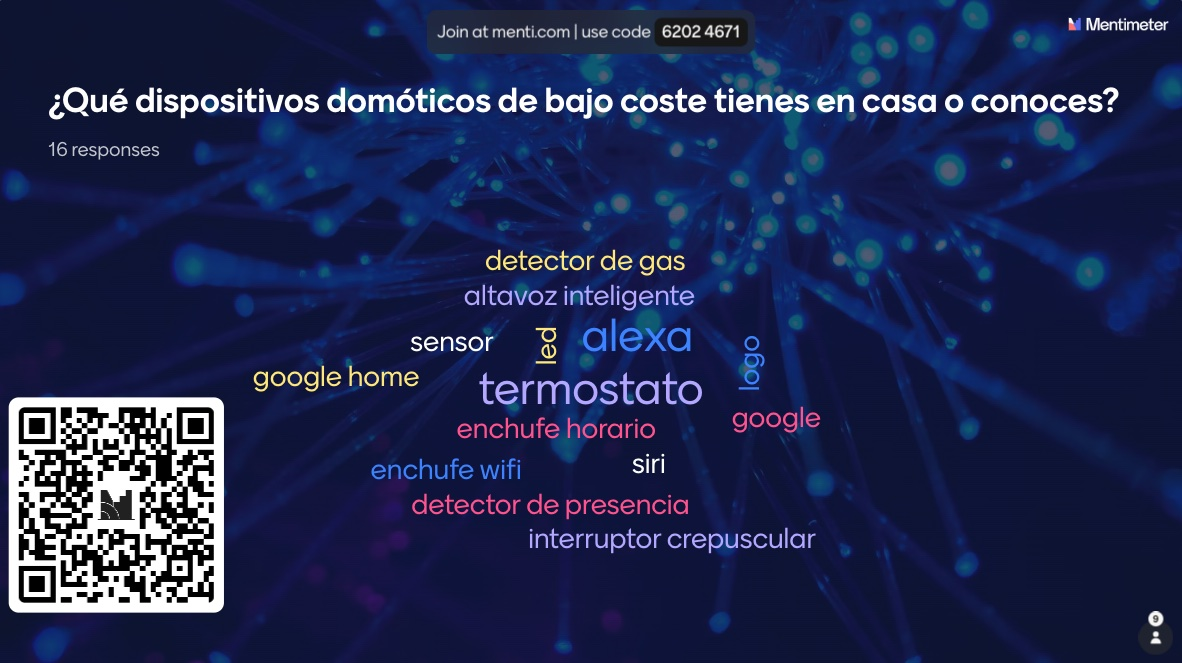
\includegraphics[width=0.8\textwidth]{resources/nube.jpg}
  \caption{Nube de palabras generada por el alumnado}
  \label{fig:nube_palabras}
\end{figure}

La actividad práctica se diseñó como una experiencia inmersiva en la que el alumnado debía simular un ataque ético. Para ello, se creó una red WiFi local con un router sin acceso a Internet, bajo el SSID “RedDomotica”, con una contraseña débil predefinida. El alumnado, trabajando en equipos, debía intentar acceder a la red, localizar un dispositivo Shelly Plug conectado, descubrir su IP y modificar su configuración sin utilizar la app oficial. 

Durante esta práctica se dieron varias situaciones destacables. Uno de los alumnos logró acceder a la configuración del router y cambió el nombre del SSID, lo que provocó que el dispositivo domótico dejara de estar accesible. Al final de la sesión, este mismo alumno se acercó a mí, algo preocupado, para confesar que había sido él quien lo había hecho, preguntando si había causado demasiados problemas. Le respondí que, si bien no era parte del plan, había sido una oportunidad valiosa para aprender de forma real y directa sobre los efectos de una mala configuración o un acceso no autorizado. 

También surgieron dificultades técnicas no previstas: no era posible acceder simultáneamente a la configuración del router desde varios dispositivos, lo cual ralentizó la actividad. Además, al intentar aplicar un ataque de fuerza bruta prolongado, el router se bloqueó temporalmente, lo que reforzó la comprensión del alumnado sobre los riesgos reales de este tipo de ataques.


% Tareas realizadas por el alumnado
\subsection{Tareas realizadas por el alumnado}

Las principales tareas que desarrolló el alumnado durante la unidad fueron:

\begin{itemize}
  \item Participación en la dinámica de nube de palabras mediante móvil y QR.
  \item Interacción durante la sesión teórica: visionado de vídeos, resolución de preguntas y debate.
  \item Acceso a la red local simulada, identificación del dispositivo conectado, análisis de su configuración y modificación del entorno.
  \item Resolución de un mini test teórico-práctico como parte de la evaluación del módulo.
\end{itemize}


% Materiales y recursos utilizados
\subsection{Materiales y recursos utilizados}

Para el desarrollo de esta unidad de trabajo se emplearon recursos didácticos, tecnológicos y materiales físicos tanto del aula como del taller del módulo de \textit{Instalaciones Domóticas}, que resultaron fundamentales para garantizar una experiencia de aprendizaje significativa y contextualizada. En un inicio, fui yo la que realizó la compra de los materiales, sin embargo, éstos no fueron utilizados, ya que el centro contaba con un router y un enchufe inteligente de la marca Shelly, que fueron los utilizados en la práctica.

Uno de los elementos clave fue el uso de un \textit{router WiFi sin conexión a Internet}, configurado previamente para crear una red local con el SSID \textit{RedDomotica}. Esta red sirvió como entorno controlado de prácticas, permitiendo que el alumnado pudiera explorar de forma segura posibles vulnerabilidades, identificar dispositivos conectados y modificar parámetros de red. La red fue diseñada con una contraseña intencionadamente débil, para facilitar la simulación de ataques de fuerza bruta y generar un contexto de reflexión sobre la importancia de una configuración segura.

El dispositivo principal de trabajo fue un \textit{enchufe inteligente Shelly Plug}, extraído del almacén del aula, junto a otros materiales domóticos disponibles en el centro. Este enchufe fue el objetivo de la práctica, permitiendo al alumnado identificar su dirección IP, acceder a su configuración y comprobar el impacto de cambios realizados desde la red local.

Además, se hizo uso de una \textit{pizarra digital interactiva SYNETECH Advance Aquarius (modelo A7532)}, adquirida recientemente por el centro gracias a fondos europeos para la modernización de la Formación Profesional. Esta herramienta facilitó la visualización de vídeos explicativos, la proyección de la presentación teórica y la generación de una \textit{nube de palabras} colaborativa a través de un código QR, permitiendo una participación dinámica e inmediata del alumnado mediante sus teléfonos móviles.

Los estudiantes utilizaron sus propios \textit{dispositivos móviles y ordenadores personales, además de los ordenadores proporcionados por el centro para los que los requerían,} para conectarse a la red local, realizar las tareas de descubrimiento y acceder a las interfaces de configuración del router y del dispositivo inteligente. Esto supuso una ventaja adicional al reproducir un entorno cercano al que podrían encontrar en un contexto doméstico real.

Por último, se diseñó una \textit{presentación en formato PDF}, que sirvió de hilo conductor para la sesión teórica. Esta incluía conceptos clave sobre seguridad, preguntas interactivas al alumnado y vídeos breves sobre vulnerabilidades en sistemas domóticos comerciales, contribuyendo a contextualizar el ejercicio práctico y fomentar una actitud crítica ante la instalación de este tipo de tecnologías.


% Criterios e instrumentos de evaluación y calificación
\section{Criterios e instrumentos de evaluación y calificación}

La evaluación de esta unidad de trabajo se diseñó conforme a un enfoque competencial, tal como establece la normativa de Formación Profesional, atendiendo no solo a la adquisición de conocimientos teóricos, sino también a la aplicación práctica, la actitud ante los retos propuestos y la reflexión crítica sobre el uso de tecnologías conectadas en red.

Los criterios de evaluación utilizados se centraron en comprobar si el alumnado era capaz de:

\begin{itemize}
  \item Reconocer riesgos de seguridad asociados a instalaciones domóticas de bajo coste.
  \item Identificar y manipular los elementos básicos de una instalación domótica (router, dispositivo conectado, red local).
  \item Aplicar medidas básicas de configuración segura, justificando sus decisiones.
  \item Verificar el funcionamiento del sistema tras la intervención.
  \item Reflexionar sobre las consecuencias de malas prácticas técnicas y éticas en entornos reales.
\end{itemize}

En cuanto a los instrumentos de evaluación, se emplearon dos. Por una parte, un análisis informal del resultado de la práctica, es decir, si el grupo había logrado acceder al dispositivo, modificar su configuración o bien reflexionar de forma crítica sobre las barreras encontradas. En este caso, no se valoró únicamente el éxito técnico, sino la comprensión del proceso y la capacidad de reflexión ante los errores. Por otra parte, se utilizó un cuestionario tipo test integrado en el examen del módulo (ver anexo \ref{examen}), que incluía tres preguntas específicas relacionadas con los contenidos y experiencias desarrolladas en la unidad. Cada pregunta valía 0,2 puntos, sumando un total de 0,6 puntos sobre la nota final del examen. Las preguntas evaluaban el conocimiento de ataques frecuentes, malas prácticas y conceptos técnicos como la escalabilidad.

Si bien no se aplicó una rúbrica formal, los criterios mencionados estuvieron presentes en el diseño de la actividad y fueron compartidos con el alumnado de manera implícita durante las explicaciones. En futuras ediciones de esta unidad se contempla la posibilidad de formalizar esta evaluación mediante rúbricas o listas de cotejo, en línea con las recomendaciones recogidas en la programación didáctica del módulo.


% Adaptaciones y atención a la diversidad
\section{Adaptaciones y atención a la diversidad}

No fue necesario aplicar adaptaciones curriculares durante esta unidad. Al tratarse de Formación Profesional, las adaptaciones curriculares de contenido no son viables, y en cuanto a las adaptaciones de acceso sólo se contemplan en casos muy concretos, y en este grupo no se dio ninguna situación que las requiriera. Sin embargo, se podría considerar como adaptación de acceso a la proporción de portátiles o materiales a los alumnos.
Tampoco se aplicaron criterios del Diseño Universal para el Aprendizaje (DUA), más allá de ofrecer información por vía visual y oral, lo cual forma parte del enfoque habitual en este tipo de módulos.

    % ANÁLISIS Y VALORACIÓN DE LA INTERVENCIÓN
\chapter{Análisis y valoración de la intervención}

\section{Reflexión sobre la intervención como docente en prácticas}

Mi participación durante el Prácticum II ha sido fundamentalmente de observación activa, aunque también he podido intervenir de forma puntual como apoyo a la docencia y, de forma más significativa, en la planificación, desarrollo y evaluación de la unidad de trabajo sobre seguridad en dispositivos domóticos. Esta intervención me ha permitido poner en práctica mis conocimientos técnicos desde una perspectiva didáctica, reflexionar sobre el funcionamiento real de un aula de Formación Profesional y adaptar mi comunicación y estrategias a un perfil de alumnado diverso.

A lo largo del periodo de prácticas, observé dinámicas muy diferentes entre los grupos, especialmente entre primer y segundo curso del ciclo de grado medio. En algunos casos, la desmotivación o el uso inadecuado del móvil dificultaban el ritmo de las clases, mientras que en otros momentos la implicación era notable, sobre todo cuando las actividades se conectaban con su entorno cotidiano o se planteaban en formato de reto.

La experiencia más significativa fue sin duda la unidad de trabajo que diseñé y llevé a cabo en el módulo de \textit{Instalaciones Domóticas}. Su planificación, desarrollo y evaluación me permitieron explorar todo el ciclo didáctico y afrontar imprevistos reales (como problemas técnicos o intervenciones espontáneas del alumnado), lo que enriqueció enormemente mi formación como futura docente.

\section{Valoración de las propuestas pedagógicas del departamento}

El Departamento de Electricidad y Electrónica muestra un compromiso activo con la mejora continua y con la aplicación de metodologías que favorezcan el aprendizaje práctico. A pesar de que el enfoque dominante sigue siendo la clase magistral tradicional, se observan esfuerzos por incorporar metodologías activas, como el aprendizaje basado en retos (ABR), especialmente en módulos como Robótica.

Sin embargo, también se detectan limitaciones estructurales y de formación docente que condicionan la implantación de enfoques más innovadores. Por ejemplo, una profesora comentó que aplicaba ABR sin haber recibido formación específica, lo que puede limitar su potencial. Aun así, se aprecia una buena disposición del profesorado a colaborar, compartir materiales y debatir sobre estrategias didácticas, lo cual es una fortaleza clara del departamento.

\section{Valoración de la programación de aula y la situación de aprendizaje}

La programación del módulo de Instalaciones Domóticas establece un marco coherente con el currículo oficial y recoge una organización de contenidos por unidades de trabajo. Mi unidad de trabajo se diseñó de forma complementaria a la programación y fue validada por el tutor, quien valoró positivamente su enfoque competencial y su conexión con temas de actualidad.

La propuesta encajó perfectamente dentro de los objetivos del módulo, trabajando competencias técnicas, actitudes profesionales y elementos transversales como la seguridad digital. La planificación fue realista en tiempos y recursos, aunque la práctica evidenció la necesidad de prever más profundamente los posibles bloqueos o problemas técnicos derivados de las condiciones del entorno (p.ej., limitaciones del router).

\section{Elaboración y uso de materiales didácticos}

Durante la intervención diseñé y utilicé una presentación propia, con estructura clara, preguntas de reflexión y vídeos breves que facilitaron el debate. También preparé un entorno de red simulado para la parte práctica, lo cual permitió reproducir un contexto de aprendizaje próximo a la realidad profesional.

Los materiales fueron bien acogidos por el alumnado, especialmente por su componente visual y participativo. Además, la nube de palabras inicial y el uso del móvil con fines académicos aportaron un valor añadido a la dinámica.

En futuras intervenciones, sería interesante sistematizar el uso de estos materiales mediante plantillas o rúbricas que permitan replicar y evaluar la experiencia con más precisión.

\section{Valoración del desarrollo de las clases}

Las sesiones se desarrollaron de forma fluida, combinando explicación teórica con actividad práctica. Se fomentó un clima participativo y respetuoso, en el que los estudiantes pudieron expresarse, proponer ideas y colaborar entre sí. Las intervenciones del alumnado fueron en general pertinentes y mostraron interés real por los aspectos técnicos de la seguridad en entornos conectados.

La sesión práctica, en concreto, generó mucho dinamismo y curiosidad. Incluso situaciones no previstas, como el cambio de SSID o el bloqueo del router, se transformaron en oportunidades de aprendizaje valiosas. Esto refuerza la idea de que el aprendizaje en FP debe estar abierto a lo imprevisto, ya que la realidad profesional no siempre sigue un guion fijo.

\section{Evaluación del aprendizaje del alumnado}

Aunque la evaluación formal se limitó a tres preguntas tipo test en el examen del módulo, la actividad permitió observar aprendizajes relevantes no siempre fácilmente evaluables. El alumnado adquirió vocabulario técnico nuevo, comprendió la importancia de la seguridad en sistemas conectados y mostró capacidad de aplicar procedimientos de configuración con criterio.

De cara a futuras intervenciones y diseño de unidades de trabajo, se podría complementar esta evaluación con una rúbrica sencilla o una autoevaluación del alumnado para recoger su percepción del aprendizaje y su implicación.

\section{Consideración sobre criterios DUA}

Durante esta unidad no se aplicaron criterios explícitos del Diseño Universal para el Aprendizaje (DUA). No obstante, sí se favoreció el acceso a la información por múltiples vías (oral, visual, práctica), se permitió el trabajo en grupo y se ofrecieron apoyos individuales durante la actividad. En un futuro, sería interesante incorporar elementos del DUA de forma más sistemática, como permitir distintas formas de expresión o adaptar tareas según niveles de dominio técnico.

\section{Propuestas y sugerencias de mejora}

A partir de esta experiencia, propongo las siguientes mejoras tanto a nivel didáctico como organizativo:

\begin{itemize}
  \item Incluir más contenidos sobre ciberseguridad en el currículo de domótica, no como unidad aislada sino de forma transversal.
  \item Facilitar formación específica al profesorado en metodologías activas como el aprendizaje basado en retos o el uso educativo de tecnologías personales.
  \item Potenciar la reflexión ética y crítica en el uso de dispositivos conectados, incluyendo casos reales, dilemas o debates.
  \item Mejorar la asignación de plazas de prácticas, procurando una correspondencia más ajustada entre el perfil del estudiante y el módulo en el que se le asigna.
  \item Documentar buenas prácticas como esta unidad de trabajo, para que puedan ser replicadas y adaptadas por otros docentes.
\end{itemize}

    % AUTOEVALUACIÓN Y CONCLUSIONES
\chapter{Autoevaluación y Conclusiones}
La experiencia me permitió conocer de cerca la FP y sus metodologías. La principal dificultad fue la desconexión entre mi formación y el contenido impartido. Aun así, logré aportar en el ámbito de la seguridad en IoT y aprender sobre gestión del aula.

\textbf{Conclusión}: El Prácticum II me ha permitido desarrollar competencias pedagógicas clave y reflexionar sobre la importancia de una mejor planificación en la asignación de prácticas.


    % Bibliografía
    \printbibliography
    \nocite{*}


    % Anexos
    \chapter*{Anexos}
    \addcontentsline{toc}{chapter}{Anexos} % Agrega "Anexos" al índice

    \appendix
    \renewcommand{\chaptername}{Anexo} % Cambia "Capítulo" por "Anexo"
    \renewcommand{\thechapter}{\Alph{chapter}} % Usa A, B, C en vez de 1, 2, 3

    \includepdf[
  pages=1,
  scale=1,
  offset=0 -3cm,
  pagecommand={
    \chapter{Presentación Sesión 6 de febrero. Domótica de Bajo Coste}
    \label{anexo:presentacion_RedDomotica}
  }
]{resources/presentacion.pdf}

\includepdf[
  pages=2-,
  scale=1
]{resources/presentacion.pdf}
    \includepdf[
  pages=1,
  scale=0.65,
  offset=0 -3cm,
  pagecommand={
    \chapter{Examen}
    \label{anexo:examen}
  }
]{resources/examen.pdf}

\includepdf[
  pages=2-,
  scale=0.65
]{resources/examen.pdf}

\end{document}










% % Intervención
% \chapter{Intervención y actuación docente en la especialidad}


%     \section{Situación de aprendizaje}
%     Elaborar e implementar una situación de aprendizaje.

%     \begin{table}[]
%         \centering
%         \begin{tabular}{| p{0.6\linewidth} | p{0.35\linewidth} |}
%         \rowcolor[HTML]{86F1E0} 
%         \hline
%         \textbf{Módulo} & \textbf{Curso/Grupo}   \\
%         \hline
%         Instalaciones Domóticas del Ciclo de Técnico de Grado Medio en Instalaciones eléctricas y automáticas (familia Electricidad y Electrónica) & 2º curso / grupo de mañana \\
%         \hline
%         \end{tabular}
%     \end{table}


%     \begin{table}[]
%       \centering
%       \begin{tabular}{| p{0.95\linewidth} |}
%       \rowcolor[HTML]{86F1E0} 
%       \hline
%       \textbf{Título de la unidad de trabajo}   \\
%       \hline
%       Domótica de bajo coste: ¿comodidad inteligente o riesgo silencioso? \\
%       \hline
%       \end{tabular}
%     \end{table}


%     \begin{table}[]
%         \centering
%         \begin{tabular}{| p{0.95\linewidth} |}
%         \rowcolor[HTML]{86F1E0} 
%         \hline
%         \textbf{Contextualización}   \\
%         \hline
%         \textbf{Entorno}: San Vicente del Raspeig es una localidad que forma parte del área metropolitana de Alicante, caracterizada por un entorno urbano a la par que un área industrial con demanda de técnicos electricistas. Además, el auge de la domótica a nivel particular, hace que se incremente la instalación de dispositivos domótcos de bajo coste en viviendas familiares sin tener en cuenta los riesgos de seguridad que puede conllevar este tipo de instalaciones.

%         \textbf{Centro educativo}: El CIPFP Canastell es un centro intregrado de ciclos de formación profesional centrado en el tejido empresarial de alrededores, en concreto en los polígonos industriales.

%         \textbf{Del alumnado y grupo-clase}: el grupo de estudiantes del módulo Instalaciones Domóticas del ciclo Instalaciones eléctricas y automáticas, turno de mañana, está compuesto por alumnado entre 17-25 años aproximadamente. El número de alumnos matriculados es de ¿28?, sin embargo, en el segundo trimestre el nivel de asistencia ha disminuido teniendo un número de presencialidad de unos 12-15 alumnos aprox. Hay alumnos que dan por perdida la asignatura aunque siguen asistiendo a clase. Otros, tienen un nivel mucho más bajo con respecto a los que van más adelantados.

%         \\
%         \hline
%         \end{tabular}
%     \end{table}


%     \begin{table}[]
%         \centering
%         \begin{tabular}{| p{0.95\linewidth} |}
%         \rowcolor[HTML]{86F1E0} 
%         \hline
%         \textbf{Justificación}   \\
%         \hline
%         Esta unidad de trabajo se centra en dar una visión actual de los riesgos de seguridad que pueden tener los dispositivos domóticos de bajo coste, analizando los posibles ataques, vulnerabilidades y cómo reducir éstos aplicando buenas prácticas. De esta forma, el alumnado puede adquirir conocimientos suficientes para asesorar a posibles clientes que les soliciten asesoramiento para realiar instalaciones domóticas.
%         \\
%         \hline
%         \end{tabular}
%     \end{table}


%     \begin{table}[]
%         \centering
%         \begin{tabular}{| p{0.95\linewidth} |}
%         \rowcolor[HTML]{86F1E0} 
%         \hline
%         \textbf{Introducción}   \\
%         \hline
        
%         \\
%         \hline
%         \end{tabular}
%     \end{table}

%     \begin{table}[]
%         \centering
%         \begin{tabular}{| p{0.95\linewidth} |}
%         \rowcolor[HTML]{86F1E0} 
%         \hline
%         \textbf{Objetivos generales}   \\
%         \hline
        
%         \\
%         \hline
%         \end{tabular}
%     \end{table}

%     \begin{table}[]
%         \centering
%         \begin{tabular}{| p{0.95\linewidth} |}
%         \rowcolor[HTML]{86F1E0} 
%         \hline
%         \textbf{Objetivos didácticos}   \\
%         \hline
        
%         \\
%         \hline
%         \end{tabular}
%     \end{table}

%     \begin{table}[]
%         \centering
%         \begin{tabular}{| p{0.95\linewidth} |}
%         \rowcolor[HTML]{86F1E0} 
%         \hline
%         \textbf{Competencias generales}   \\
%         \hline
        
%         \\
%         \hline
%         \end{tabular}
%     \end{table}

%     \begin{table}[]
%         \centering
%         \begin{tabular}{| p{0.95\linewidth} |}
%         \rowcolor[HTML]{86F1E0} 
%         \hline
%         \textbf{Competencias profesionales, personales y sociales}   \\
%         \hline
        
%         \\
%         \hline
%         \end{tabular}
%     \end{table}

%     \begin{table}[]
%         \centering
%         \begin{tabular}{| p{0.95\linewidth} |}
%         \rowcolor[HTML]{86F1E0} 
%         \hline
%         \textbf{Resultados de aprendizaje}   \\
%         \hline
        
%         \\
%         \hline
%         \end{tabular}
%     \end{table}

%     \begin{table}[]
%         \centering
%         \begin{tabular}{| p{0.95\linewidth} |}
%         \rowcolor[HTML]{86F1E0} 
%         \hline
%         \textbf{Criterios de evaluación}   \\
%         \hline
        
%         \\
%         \hline
%         \end{tabular}
%     \end{table}

%     \begin{table}[]
%         \centering
%         \begin{tabular}{| p{0.95\linewidth} |}
%         \rowcolor[HTML]{86F1E0} 
%         \hline
%         \textbf{Contenidos}   \\
%         \hline
        
%         \\
%         \hline
%         \end{tabular}
%     \end{table}

%     \begin{table}[]
%         \centering
%         \begin{tabular}{| p{0.95\linewidth} |}
%         \rowcolor[HTML]{86F1E0} 
%         \hline
%         \textbf{Elementos transversales}   \\
%         \hline
        
%         \\
%         \hline
%         \end{tabular}
%     \end{table}

%     \begin{table}[]
%         \centering
%         \begin{tabular}{| p{0.95\linewidth} |}
%         \rowcolor[HTML]{86F1E0} 
%         \hline
%         \textbf{Metodología}   \\
%         \hline
        
%         \\
%         \hline
%         \end{tabular}
%     \end{table}

%     \begin{table}[]
%         \centering
%         \begin{tabular}{| p{0.95\linewidth} |}
%         \rowcolor[HTML]{86F1E0} 
%         \hline
%         \textbf{Sesión}   \\
%         \hline
        
%         \textbf{Objetivo de la sesión}: \\

%         \textbf{Duración}: \\

%         \textbf{Actividades}:
%         \begin{itemize}
%             \item \textbf{Actividad 1}: Presentación de conceptos, características de los dispositivos domóticos de bajo coste, reflexión sobre vulnerabiidades y consejos básicos para reducir riesgos. Será un trabajo en grupo-clase donde todo el alumnado participará en las reflexiones y cuestiones planteadas. La presentación será proyectada en la pizarra electrónica, teniendo varios puntos de interacción con el alumando para mantener el interés y la atención: al inicio de la presentación, y a modo de rompehielo, se utilizará un código QR a través del cual los alumnos podrán participar en una nube de palabras a través de su dispositvo móvil; en otro momento, se lanzarán interrogantes sobre cuestiones relacionadas con los riesgos de seguridad y saldrán a la pizarra para apuntar lo que se les ha ocurrido.

%             \item \textbf{Actividad 2}: Actividad Práctica de una instalación domótica básica. Con unos pocos dispositivos (como un router, y una bombilla inteligente o similar) se intentará configurar una red simulando una red insegura donde los alumnos podrán "hackear" la red y aprender por qué es importante tener en consideración los aspectos de seguridad. Intentarás conectar la bombilla inteligente a la red, pasando por la instalación de la app correspondiente que les solicitará permisos de WiFi, Bluetooth, Localización, etc. Se realizará con un móvil que no sea del propio alumnado para no comprometer su provacidad. De esta forma, podrán analizar y reflexionar sobre por qué pueden estas aplicaciones solicitar dichos datos, si son seguros, si respetan la privacidad, etc.
%             \begin{itemize}
%                 \item \textbf{Prueba 1}: router huawei (vodafone 2012) no conectado a Internet, configurado con un SSID denominado "RedDomotica" con contraseña débil (12345678). Bombilla inteligente y enchufe inteligente obramart. 
%                 \begin{itemize}
%                     \item Instalación de la app Tuya Smart (se requiere registro)
%                     \item Instalación de la app NavigationSmartHome (para la bombilla) (se requiere registro)
%                     \item La instalación de las app requiere acceso a WiFi, Bluetooth y Localización.
%                     \item El móvil se conecta a la red RedDomotica, la cual no tiene acceso a Internet.
%                     \item Se enciende el dispositivo, primero la bombilla y luego el enchufe por separado. Con el móvil conectado a la red 
%                 \end{itemize}

%                 \item \textbf{Prueba 2}: router huawei (vodafone 2012) configurado como switch, con el mismo SSID y mismo password, ahora con acceso a Internet. Bombilla inteligente y enchufe inteligente obramart. 
%                 \begin{itemize}
%                     \item Instlada la app Tuya Smart
%                     \item El móvil se conecta a la red RedDomotica, la cual no tiene acceso a Internet.
%                     \item Misma operación que en el caso anterior. Parece ser que el indicador de progreso avanza algo más, pero falla igualmente el emparejamiento.
%                 \end{itemize} 

%                 \item \textbf{Prueba 3}:  router tp-link. Configurado con SSID "RedDomotica" y contraseña débil, sin acceso a Internet. Enchufe inteligente Selly Plug y app de la misma marca. 
%                 \begin{itemize}
%                     \item Instalación de la app Shelly (requiere registro: creación de la cuenta clasedomotica6@gmail.com - Qwerty12345!)
%                     \item Se conecta el enchufe inteligente a la corriente. 
%                     \item Se conecta el móvil a RedDomotica
%                     \item Se intenta asignar la red RedSomotica al enchufe.
%                 \end{itemize} 
%             \end{itemize}

%         \end{itemize}
%         \\
%         \hline
%         \end{tabular}
%     \end{table}

% % Autoevaluación y conclusiones
% \chapter{Autoevaluación y Conclusiones}

% % Bibliografía
% \chapter*{Bibliografía}
% \begin{itemize}
%   \item CIPFP Canastell. "Organización del centro". Recuperado de: \url{https://portal.edu.gva.es/cipfpcanastell/informacion-general/organizacion-del-centro/}
%   \item Proyecto de Dirección CIPFP Canastell 2022-2026. Documento interno del centro.
% \end{itemize}



% \end{document}
